%% LaTeX-Beamer template for KIT design
%% by Erik Burger, Christian Hammer
%% title picture by Klaus Krogmann
%%
%% version 2.1
%%
%% mostly compatible to KIT corporate design v2.0
%% http://intranet.kit.edu/gestaltungsrichtlinien.php
%%
%% Problems, bugs and comments to
%% burger@kit.edu

\documentclass[18pt]{beamer}
\usepackage[utf8]{inputenc}
\usepackage{listings}
\usepackage{tikz}
%% SLIDE FORMAT

% use 'beamerthemekit' for standard 4:3 ratio
% for widescreen slides (16:9), use 'beamerthemekitwide'

\usepackage{templates/beamerthemekit}
% \usepackage{templates/beamerthemekitwide}

%% TITLE PICTURE

% if a custom picture is to be used on the title page, copy it into the 'logos'
% directory, in the line below, replace 'mypicture' with the 
% filename (without extension) and uncomment the following line
% (picture proportions: 63 : 20 for standard, 169 : 40 for wide
% *.eps format if you use latex+dvips+ps2pdf, 
% *.jpg/*.png/*.pdf if you use pdflatex)

\titleimage{banner}

%% TITLE LOGO

% for a custom logo on the front page, copy your file into the 'logos'
% directory, insert the filename in the line below and uncomment it

\titlelogo{logo}

% (*.eps format if you use latex+dvips+ps2pdf,
% *.jpg/*.png/*.pdf if you use pdflatex)

%% TikZ INTEGRATION

% use these packages for PCM symbols and UML classes
% \usepackage{templates/tikzkit}
% \usepackage{templates/tikzuml}

% the presentation starts here

\title[Vortrag Geometrie I]{Geometrie I}
\subtitle{Problemstellungen in 0 bis 3 Dimensionen}
\author{Lukas Böhm, Eric Sallermann, Vincent Schüßler}

\institute{ICPC Basispraktikum SS2014}

\beamertemplatenavigationsymbolsempty

% custom commands
\newcommand{\anf}[1]{\glqq#1\grqq}
\newcommand{\norm}[1]{\left\|#1\right\|} 
\usetikzlibrary{arrows}

% Zeichenbereich
\tikzstyle{every picture}=[domain=0:4]
% Gitterstil. Zum Stil ’help lines’ wird Linienart ’dotted’ hinzugefügt
\tikzstyle{help lines}+=[dotted]

\begin{document}

% change the following line to "ngerman" for German style date and logos
\selectlanguage{ngerman}

%title page
\begin{frame}
\titlepage
\end{frame}

%table of contents
%~ \begin{frame}{Übersicht}
%~ \tableofcontents
%~ \end{frame}

\begin{frame}{Floating Point Beispiel}
	\lstset{
		language=C++,
		tabsize=2
	}
	\lstinputlisting{error.cpp}
	Ausgabe?
\end{frame}

\begin{frame}{Unerwartete Ergebnisse}
	\begin{exampleblock}{Ausgabe}
		3.5999999046325683594 \\
		false\\
		false
	\end{exampleblock}
	3.6 nicht darstellbar \\
	Rundungsfehler \\
	Seltsame Sonderwerte:
	\begin{itemize}
		\item NaN
		\item Inf
		\item +-0
	\end{itemize}
\end{frame}

\begin{frame}{IEEE 754 Knigge}
	\begin{itemize}
		\item Floats \& Doubles möglichst vermeiden
		\item Wenn nötig, erst ganz spät von Ganzzahl zu Fließkomma wechseln
		\item Bitte KEIN float und NUR double benutzen
		\item Keine direkten Vergleiche
	\end{itemize}

\end{frame}

\begin{frame}{Vektoren - Einführung}
	\begin{center}
		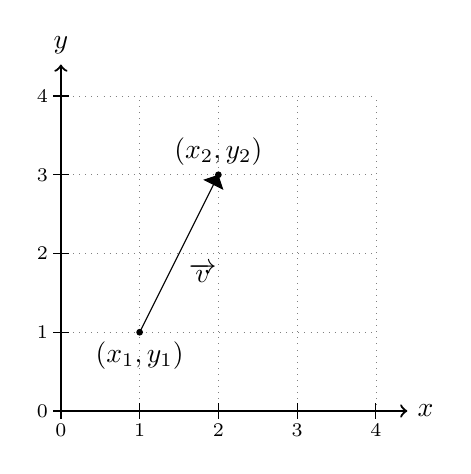
\begin{tikzpicture}[scale=1]
			% Gitter zeichnen
			\draw[style=help lines,step=1cm] (0,0) grid (4,4);
			% Achsen zeichnen
			\draw[->,thick] (-0.1,0) -- (4.4,0) node[right] {$x$};
			\draw[->,thick] (0,-0.1) -- (0,4.4) node[above] {$y$};
			% Punkte zeichnen
			\filldraw (1,1) circle (1pt) node[below] {$(x_1,y_1)$};
			\filldraw (2,3) circle (1pt) node[above] {$(x_2,y_2)$};
			% Vektor zeichnen
			\draw[-triangle 90] (1,1) -- (2,3) node[midway, anchor=north west] {$\overrightarrow{v}$};
			% Achsen beschriften
			\foreach \x in {0,1,2,3,4}
				\draw (\x,-.1) -- (\x,.1) node[below=4pt] {$\scriptstyle\x$};
			\foreach \y in {0,1,2,3,4}
				\draw (-.1,\y) -- (.1,\y) node[left=4pt] {$\scriptstyle\y$};
		\end{tikzpicture}
	\end{center}

	\begin{itemize}
		\item Definiert durch zwei Punkte und eine \anf{Richtung}
		\item $\overrightarrow{v} = \left(\begin{array}{c} x_2 \\ y_2 \end{array}\right) - \left(\begin{array}{c} x_1 \\ y_1 \end{array}\right) = \left(\begin{array}{c} x_2 - x_1 \\ y_2 - y_1 \end{array}\right) = \left(\begin{array}{c} dx \\ dy \end{array}\right)$
	\end{itemize}
\end{frame}

\begin{frame}{Vektoren - Einführung}
	\begin{block}{Skalieren eines Vektors}
		$\lambda * \overrightarrow{v} := \left(\begin{array}{c} \lambda * x \\ \lambda * y \end{array}\right)$ \\
		Für $\lambda \in (0, 1)$ wird $\overrightarrow{v}$ kürzer,\\
		für $\lambda = 1$ behält $\overrightarrow{v}$ seine Länge bei,\\
		für $\lambda > 1$ wird $\overrightarrow{v}$ länger.
	\end{block}
	\begin{block}{Verschieben eines Punktes um einen Vektor}
		$P + \overrightarrow{v} := \left(\begin{array}{c} P_x \\ P_y \end{array}\right) + \left(\begin{array}{c} v_x \\ v_y \end{array}\right) = \left(\begin{array}{c} P_x + v_x \\ P_y + v_y \end{array}\right)$
	\end{block}
\end{frame}

\begin{frame}{Vektoren - Einführung}
	Skalierung
	\begin{center}
		\begin{tikzpicture}[scale=1]
			% Gitter zeichnen
			\draw[style=help lines,step=1cm] (0,0) grid (4,4);
			% Achsen zeichnen
			\draw[->,thick] (-0.1,0) -- (4.4,0) node[right] {$x$};
			\draw[->,thick] (0,-0.1) -- (0,4.4) node[above] {$y$};
			% Punkte zeichnen
			\filldraw (1,1) circle (1pt);
			% Vektor zeichnen
			\draw[-triangle 90] (1.5,2) -- (2,3) node[midway, anchor=north west] {$\overrightarrow{v}$};
			\draw[draw=red,-triangle 90, fill=red] (1,1) -- (1.5,2) node[midway, anchor=north west] {$\frac{1}{2} * \overrightarrow{v}$};
			% Achsen beschriften
			\foreach \x in {0,1,2,3,4}
				\draw (\x,-.1) -- (\x,.1) node[below=4pt] {$\scriptstyle\x$};
			\foreach \y in {0,1,2,3,4}
				\draw (-.1,\y) -- (.1,\y) node[left=4pt] {$\scriptstyle\y$};
		\end{tikzpicture}
	\end{center}
\end{frame}

\begin{frame}{Vektoren - Einführung}
	Verschiebung
	\begin{center}
		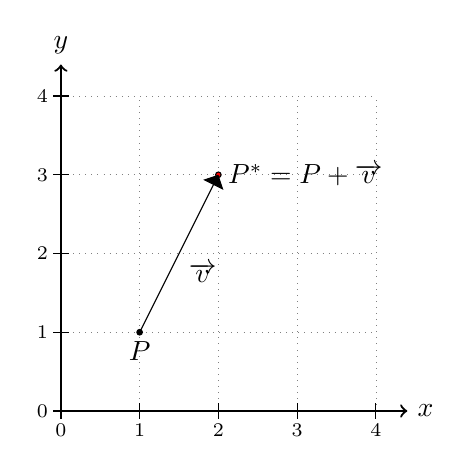
\begin{tikzpicture}[scale=1]
			% Gitter zeichnen
			\draw[style=help lines,step=1cm] (0,0) grid (4,4);
			% Achsen zeichnen
			\draw[->,thick] (-0.1,0) -- (4.4,0) node[right] {$x$};
			\draw[->,thick] (0,-0.1) -- (0,4.4) node[above] {$y$};
			% Punkte zeichnen
			\filldraw (1,1) circle (1pt) node[below] {$P$};
			\filldraw[fill=red] (2,3) circle (1pt) node[right] {$P^* = P + \overrightarrow{v}$};
			% Vektor zeichnen
			\draw[-triangle 90] (1,1) -- (2,3) node[midway, anchor=north west] {$\overrightarrow{v}$};
			% Achsen beschriften
			\foreach \x in {0,1,2,3,4}
				\draw (\x,-.1) -- (\x,.1) node[below=4pt] {$\scriptstyle\x$};
			\foreach \y in {0,1,2,3,4}
				\draw (-.1,\y) -- (.1,\y) node[left=4pt] {$\scriptstyle\y$};
		\end{tikzpicture}
	\end{center}
\end{frame}

\begin{frame}{Vektoren - Einführung}
	\begin{block}{Länge eines Vektors}
		Die Länge eines Vektors hängt von der verwendeten Norm $\norm{\cdot}$ ab,\\
		überlicherweise verwenden wir die {\bf Euklische Norm} $\norm{\cdot}_2$ .\\
		Im zweidimensionalen Fall ist sie definiert als\\
		$\norm{\left(\begin{array}{c} x \\ y \end{array}\right)}_2 := \sqrt{x^2 + y^2}$
	\end{block}
\end{frame}

\begin{frame}{Vektoren - Skalarprodukt}
	\begin{block}{Skalarprodukt zweier Vektoren im kartesischen Koordinatensystem}
		$\left(\begin{array}{c} a_x \\ a_y \end{array}\right) \cdot \left(\begin{array}{c} b_x \\ b_y \end{array}\right) := a_x * b_x + a_y * b_y$
	\end{block}
	
	Anschaulich betrachtet liefert das Skalarprodukt der Vektoren $\overrightarrow{a}$ und $\overrightarrow{b}$ einen Wert
	\begin{itemize}
		\item $< 0$, wenn $\overrightarrow{a}$ und $\overrightarrow{b}$ einen stumpfen Winkel ($> 90^{\circ}$) bilden,
		\item $= 0$, wenn $\overrightarrow{a}$ und $\overrightarrow{b}$ rechtwinklig aufeinander stehen und
		\item $> 0$, wenn $\overrightarrow{a}$ und $\overrightarrow{b}$ einen spitzen Winkel ($< 90^{\circ}$) bilden.
	\end{itemize}
\end{frame}

\begin{frame}{Vektoren - Kreuzprodukt}
	\begin{block}{Kreuzprodukt zweier Vektoren im zweidimensionalen Fall}
		$\left(\begin{array}{c} a_x \\ a_y \end{array}\right) \times \left(\begin{array}{c} b_x \\ b_y \end{array}\right) := a_x * b_y - a_y * b_x$
	\end{block}
	
	\begin{itemize}
		\item Überlicherweise nur im dreidimensionalen Raum definiert. Das Ergebnis ist ein Vektor, der orthogonal auf beide Eingabevektoren steht.
		\item Im zweidimensionalen Fall liefert das Kreuzprodukt die {\bf Z-Koordinate} eines orthogonalen Vektors, der entlang der Z-Achse zeigt.
		\item Länge dieses Vektors entspricht dem Flächeninhalt des Parallelogramms mit $\overrightarrow{a}$ und $\overrightarrow{b}$ als Seiten.
	\end{itemize}
\end{frame}

\begin{frame}{Vektoren - Kreuzprodukt}
	\begin{center}
		(Animation)\\
		Quelle:	\url{http://upload.wikimedia.org/wikipedia/commons/6/6e/Cross_product.gif}
	\end{center}
\end{frame}

\begin{frame}{Linksknick-Test/CCW-Test}
	Anhand unserer bisherigen Ergebnisse können wir nun ganz einfach einen Linksknick-Test generieren.
	
	\begin{block}{Linksknick-Test}
		\textit{Gegeben:} Drei Punkte $p$, $q$ und $r$.\\ \ \\
		
		Bilde die Vektoren $\overrightarrow{pq}$ und $\overrightarrow{pr}$. Berechne das Kreuzprodukt $\tau = \overrightarrow{pq} \times \overrightarrow{pr}$. Der Streckenzug $p \rightarrow q \rightarrow r$ bildet,\\
		falls $\tau < 0$, einen Rechtsknick,\\
		bei $\tau = 0$ sind die Strecken koolinear, und\\
		falls $\tau > 0$, einen Linksknick.\\ \ \\
		
		Wenn also $\tau > 0$ gilt, so ist $p \rightarrow q \rightarrow r$ ein Linksknick.
	\end{block}
\end{frame}

\begin{frame}{Vektoren - Einführung - Code}
	\lstset{
		language=C++,
		tabsize=1
	}
	\lstinputlisting[firstline=1, lastline=14]{vectors.cpp}
\end{frame}

\begin{frame}{Vektoren - Einführung - Code}
	\lstset{
		language=C++,
		tabsize=1
	}
	\lstinputlisting[firstline=16, lastline=29]{vectors.cpp}
\end{frame}

\begin{frame}{Vektoren - Skalarprodukt/Kreuzprodukt - Code}
	\lstset{
		language=C++,
		tabsize=1
	}
	\lstinputlisting[firstline=31, lastline=39]{vectors.cpp}
\end{frame}

\begin{frame}{Linksknick-Test/CCW-Test - Code}
	\lstset{
		language=C++,
		tabsize=1
	}
	\lstinputlisting[firstline=41, lastline=49]{vectors.cpp}
\end{frame}

\begin{frame}{Polygone}
	\begin{itemize}
		\item Definition
		\item Konvex/Konkav
		\item Repräsentation
	\end{itemize}
\end{frame}

\begin{frame}{Flächeninhalt von Polygonen}
	\begin{itemize}
		\item Wie groß ist der Flächeninhalt eines Polygons?
		\item Formel für Flächeninhalt
		\item Visualisierung auf Bild
	\end{itemize}
\end{frame}

\begin{frame}{Überprüfung von Konvexität}
	\begin{itemize}
		\item Ist das Polygon konvex?
		\item CCW für alle Eckpunkte mit Nachbarn
		\item (kurzer Pseudocode)
		\item Beispiel für jeweils Konvex/Konkav
	\end{itemize}
\end{frame}

\begin{frame}{Punkt in Polygon}
	\begin{itemize}
		\item Liegt ein Punkt in einem Polygon?
		\item Winkel zwischen benachbarten Eckpunkten und Punkt aufsummieren
		\item (kurzer Pseudocode)
		\item Beispiel für innen/außen
	\end{itemize}
\end{frame}


\end{document}
